\section{Matched Filtering, Signal-to-Noise Ratio, And $\chi$ Square} \label{sec:6}

\subsection{Matched Filtering}

We apply frequency-domain matched filtering to the H1 strain data
using waveform templates generated with the IMRPhenomD approximant.
The matched-filter SNR is defined by the noise-weighted inner product.

\begin{equation}
	(a|b) = 4 \, \Re \int_{0}^{\infty}
	\frac{\tilde{a}(f)\tilde{b}^*(f)}{S_n(f)} \, df ,
\end{equation}

where $S_n(f)$ is the one-sided power spectral density (PSD) and $\tilde{a(f)}, \tilde{b^*(f)}$ are representing detector and model data in frequency. 
The time-dependent SNR is

\begin{equation}
	\rho(t) = \frac{(s|h_t)}{\sqrt{(h|h)}} ,
\end{equation}

with $h_t$ the time-shifted template.
Inverse PSD weighting suppresses noisy frequency bands and
optimally accumulates signal power in the sensitive band
(20--300 Hz). This procedure is just like whitening data.
SNR is just: weighted dot product of signal and template.

But in discrete form the matched-filter SNR is defined:
\begin{equation}
	(a|b) = 4 \Re \sum_{k} \frac{\tilde{a}_k \tilde{b}_k^*}{S_n(f_k)} \Delta f .
\end{equation}
When we convert time-series data to frequency domain using FFT, we do not get continuous frequencies.
We get discrete frequency bins $f_k = k \Delta f$. and $\Delta f$ is resolution of our FFT and it relates to segment length. it could be calculated by dividing sample rate by length of data. 
 
\subsection{Chi-Square Signal Consistency Test}
To test waveform consistency, we compute the
power $\chi^2$ discriminator \cite{Allen2005Chisq}.
The template is divided into $p$ frequency bins,
and deviations of observed power from the expected template
distribution are measured:

\begin{equation}
	\chi^2(t) = \sum_{k=1}^{p} {\left| \rho_k(t) - \frac{\rho(t)}{p} \right|^2} ,
\end{equation}
where $\rho_k(t)$ is SNR contribution from bin k and $\rho(t)$ is total SNR. In above equation we just compare SNR of each bin with SNR that it is distributed equally between all bins. 
with degrees of freedom
\begin{equation}
	\mathrm{DOF} = 2p - 2 .
\end{equation}
we can define and use $\chi^2_{reduced}$
\begin{equation}
	\chi^2_{\mathrm{red}} = \frac{\chi^2}{\mathrm{DOF}} .
\end{equation}
In our processing if $\chi^2_{red}$ is between 1 and 2 our signal is very good.

\subsection{Reweighted SNR}

Following standard LIGO practice \cite{Allen2005Chisq, Abbott2016Discovery},
we compute the reweighted SNR:
\begin{equation}
	\hat{\rho} =
	\begin{cases}
		\rho & \text{if } \chi^2_{\mathrm{red}} \le 1, \\
		\displaystyle
		\frac{\rho}{\left[\frac{1 + (\chi^2_{\mathrm{red}})^3}{2}\right]^{1/6}}
		& \text{if } \chi^2_{\mathrm{red}} > 1.
	\end{cases}
\end{equation}

This suppresses triggers caused by noise transients that
produce large $\chi^2$ values.

\subsection{Parameter Optimization And Final Results}

We explored a small grid around the expected GW150914 masses:

\[
(m_1, m_2) \in
\{(35.5,30.5), (36,30), (36.5,30), (36,30.5), (35,30)\} M_\odot
\]

and tested $p = 16, 26, 36$ $\chi^2$ bins. The smallest reduced $\chi^2$ was obtained for:

\begin{table}[h]
	\centering
	\begin{tabular}{ll}
		$m_1 = 35.5 M_\odot$          & $\chi^2 = 147.01$ \\
		$m_2 = 30.5 M_\odot$          & Reduced $\chi^2 = 2.10$ \\
		$p = 36$ bins                 & Reweighted SNR: $\hat{\rho} = 13.31$ \\
		Peak SNR: $\rho = 17.48$      & Time offset: $29.20$ ms \\
	\end{tabular}
\end{table}
with total mass $66.0 M_\odot$ and mass ratio $q = 1.16$.

\begin{figure}[h]
	\centering
	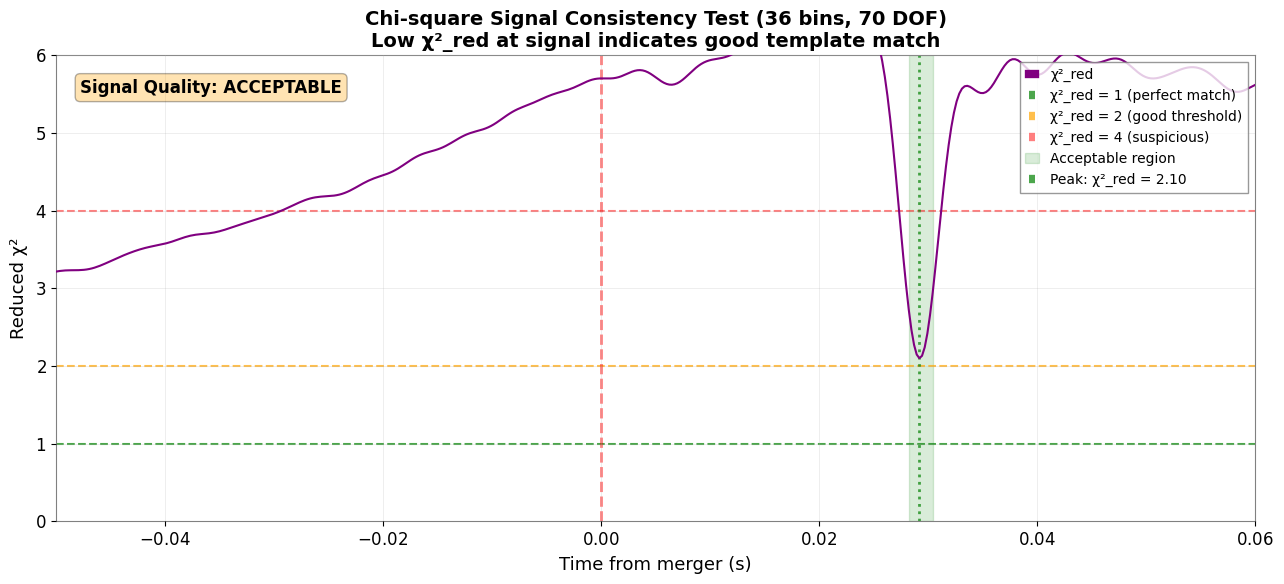
\includegraphics[width=0.9\textwidth]{figure/reduced_chi_time.png}
	\caption{$\chi^2_{red}$ over time near merger.}
	\label{chi2}
\end{figure}

The reduced $\chi^2$ indicates moderate deviation from a
perfect template match but remains within acceptable limits.
The reweighted SNR of $\hat{\rho} \approx 13.3$
corresponds to a detection significance of approximately
$13\sigma$ in Gaussian noise.
\begin{figure}[h]
	\centering
	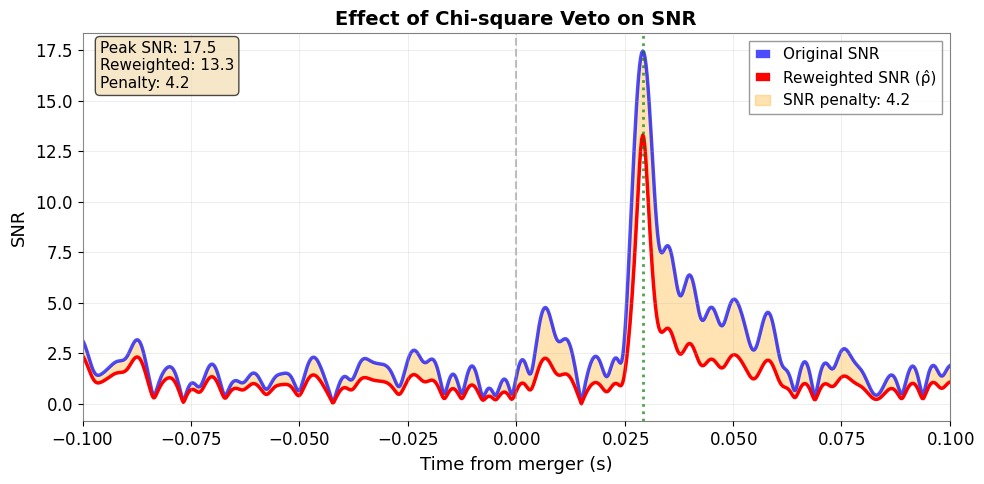
\includegraphics[width=0.9\textwidth]{figure/SNR.png}
	\caption{SNR over time near merger.}
	\label{SNR}
\end{figure}

As we see in figure \ref{chi2} and \ref{SNR}, the SNR peak completely match with best value of $\chi^2$. The "offset" refers to the time difference between where we expected the merger to occur and where we actually detected the peak signal. And For GW150914:
\begin{itemize}
	\item The entire inspiral-merger-ringdown signal lasts ~0.2 seconds
	\item A 30ms offset is only 0.15 of the total signal duration
	\item LIGO's timing accuracy is ~1-10 milliseconds, so 30ms is reasonable	
\end{itemize}
There is a offset because the merger time is not necessarily the exact moment of peak amplitude so different conventions exist for defining "merger time". Besides that IMRPhenomD is just an approximate model.

These results are consistent with the published
GW150914 analysis and confirm the astrophysical
origin of the signal.
